\documentclass[10pt,xcolor=dvipsnames,italian]{beamer}

% Preambolo del documento
%****************************************************************************************************
% PACCHETTI
%****************************************************************************************************
% Tema principale
%\usetheme{Mainz}

%\usepackage{fontspec}
%\usepackage[libertine={Ligatures=TeX,RawFeature=+onum},biolinum={Ligatures=TeX,RawFeature=+onum}]{libertineotf}

\usepackage[biolinum,sfdefault]{libertine}
\usepackage{eulervm}

\usepackage[italian]{babel}

\usepackage[T1]{fontenc}
\usepackage[utf8]{inputenc}

%\usepackage{beamerfoils}
%\usepackage{array}
%\usepackage{mathrsfs}
\usepackage{booktabs}
\usepackage{color}
\usepackage{colortbl}    
\usepackage[version=3]{mhchem} 
%\usepackage{gensymb}
\usepackage{tabularx}
%\usepackage{cancel}
\usepackage[labelformat=empty,labelsep=none,skip=1pt]{caption}
\usepackage[per-mode=symbol]{siunitx}
\usepackage{relsize,xspace}
\usepackage{bm}
\usepackage{pgfpages}

\usepackage{tikz}
\usetikzlibrary{shapes,arrows,shadows,mindmap,trees,calc}

\usepackage{lipsum}

%****************************************************************************************************

%\setbeamercovered{dynamic}

\def\arrowd{
  (10.75:1.1) -- (6.5:1) arc (6.25:120:1) [rounded corners=0.5] --
  (120:0.9) [rounded corners=1] -- (130:1.1) [rounded corners=0.5] --
  (120:1.3) [sharp corners] -- (120:1.2) arc (120:5.25:1.2)
  [rounded corners=1] -- (10.75:1.1) -- (6.5:1) -- cycle
}

\tikzset{
  ashadow/.style={opacity=.25, shadow xshift=0.07, shadow yshift=-0.07},
}


%****************************************************************************************************
% COLORI e STILI di TESTO
\definecolor{greendark}{RGB}{0,178,140}
\definecolor{bluegreen}{cmyk}{0.9,0.0,0.35,0.2}
\definecolor{darkblue}{rgb}{0.2,0.2,0.65}
\definecolor{themecolor}{rgb}{0.137,0.466,0.741} % blue


%\newcommand{\cit}{\scriptsize\color{bluegreen}}             % citazioni
\newcommand{\cit}{\scriptsize\color{themecolor!80!green}}             % citazioni
\newcommand{\tbtit}{\bf\color{themecolor!75!black}} % titoli nelle tabelle
\newcommand{\ev}{\color{themecolor}\bf}
%\renewcommand{\CancelColor}{\color{red}}
%****************************************************************************************************


%****************************************************************************************************
% TABELLE
\newcolumntype{C}[1]{>{\centering\let\newline\\\arraybackslash\hspace{0pt}}m{#1}}
\setlength{\aboverulesep}{0pt}
\setlength{\belowrulesep}{0pt}
\setlength{\extrarowheight}{.75ex}
\arrayrulecolor{themecolor!75!black}

\newcommand{\tabitem}{~~\llap{\textbullet}~~}
%****************************************************************************************************


%****************************************************************************************************
% FRECCE
\tikzset{bluearrow/.style={draw=themecolor,fill=themecolor,single arrow,drop shadow=%
                           {shadow xshift=.3ex,shadow yshift=-.3ex,color=themecolor!60!black},
                           minimum height=3.5ex,minimum width=0.1ex,single arrow head extend=0.5ex,
                           single arrow tip angle=70}}

\newcommand{\arrowup}{\tikz[baseline=-0.5ex]{\node[bluearrow,rotate=90]{};}}
\newcommand{\arrowdown}{\tikz[baseline=-0.5ex]{\node[bluearrow,rotate=-90]{};}}
\newcommand{\arrowright}{\tikz[baseline=-0.5ex]{\node[bluearrow]{};}}
\newcommand{\arrowleft}{\tikz[baseline=-0.5ex]{\node[bluearrow,rotate=180]{};}}
%****************************************************************************************************


% COMANDI PERSONALI
\newcommand{\gete}{\ce{GeTe}\xspace}

% Path per le immagini
\graphicspath{{Immagini/}{../Thesis/Immagini/Plots/}{../THESIS/Immagini/}{../THESIS/Immagini/Plots/}{../THESIS/Immagini/bulk_figures/}}



% Titolo, autore, institution
\title[Cristallizzazione in nanofili di \gete]{Simulazioni atomistiche del processo di cristallizzazione in nanofili di \gete}
%\author[Edoardo Baldi]{\vspace{-3ex}\\Silvia Gabardi\\ \vspace{2ex} Supervisor: Prof. M. Bernasconi}
\author[Edoardo Baldi]{Edoardo Baldi \\\medskip {\small\emph{Relatore:} Prof.~Marco~Bernasconi}}
\date[]{23 Marzo 2015}
\institute[Università di Milano--Bicocca]{Università di Milano--Bicocca --- Dipartmento di Fisica}
%\logo{\includegraphics[angle=0,width=0.1\paperwidth]{Logo_Green}}

%**************************************************
% INIZIO DOCUMENTO %
%**************************************************

\begin{document}

\tikzstyle{cloud}=[draw,ellipse,fill=blue!20]%,node distance=3cm,minimum height=2em]

\begin{frame}
\titlepage
\end{frame}
\LogoOff


\end{document}

%**************************************************************

\section{Introduction}

\begin{frame}
\frametitle{Phase change materials for optical and electronic memories}
\begin{minipage}{1.0\textwidth}
  \begin{minipage}[b]{0.53\linewidth}
  Optical memories: DVD
  \end{minipage}
\hfill
  \begin{minipage}[b]{0.43\linewidth}\centering
  \includegraphics[angle=0, width=0.4\textwidth]{DVD.eps}
  \end{minipage}
\end{minipage}
\begin{minipage}{1.0\textwidth}
  \begin{minipage}[b]{0.53\linewidth}
  Non-volatile electronic memories:\hfill\\ Phase Change Memories (PCM)
  \end{minipage}
\hfill
  \begin{minipage}[b]{0.43\linewidth}\centering
  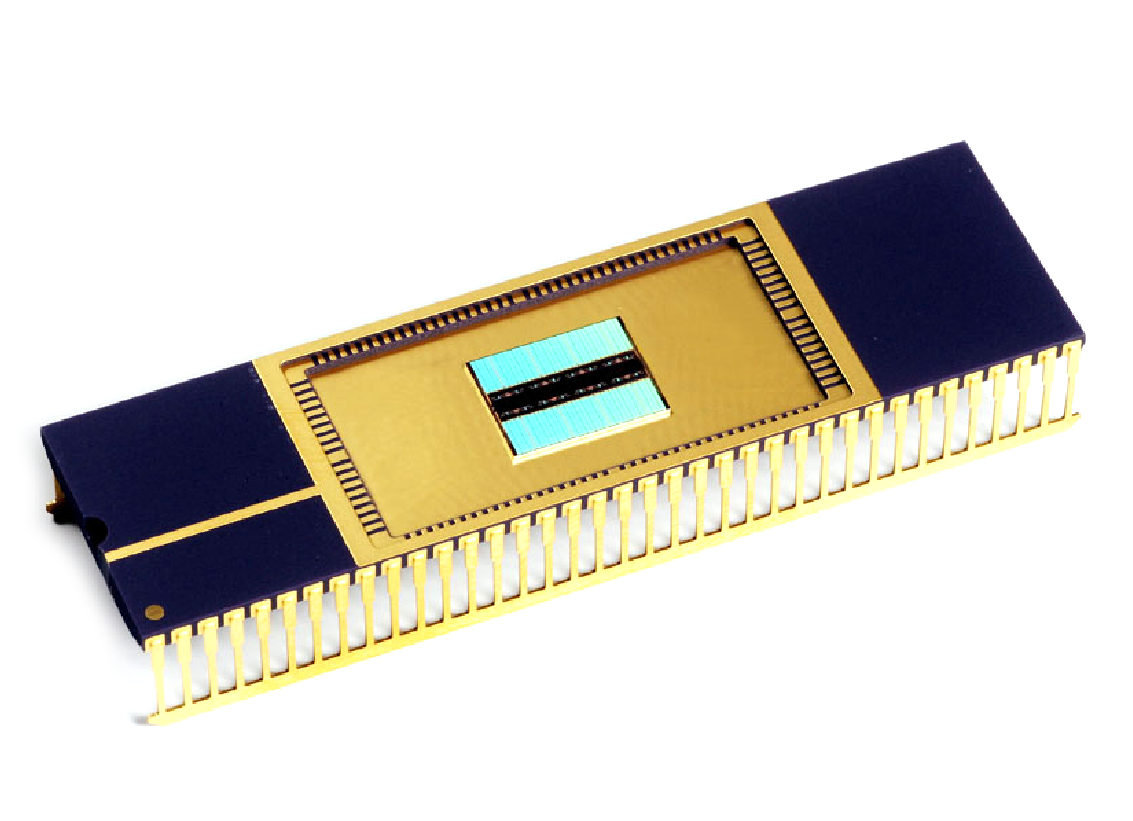
\includegraphics[angle=0, width=0.4\textwidth]{PCM.eps}\\
  \end{minipage}
\end{minipage}
\vspace{1cm}\\
%\onslide<2->{
Chalcogenide alloys: {\ev GeTe}, \textcolor{themecolor}{\textbf{Ge$_2$Sb$_2$Te$_5$ (GST)}}\\
\vspace{0.5cm}
fast and reversible amorphous-to-crystal phase transition (50~ns)\\
%}
\end{frame}

\note{
Phase Change materials are of great technological importance in the realization of
non\---volatile memories the rewritable DVDs and electronic
memories of new concept named Phase Change Memories.\\
For electronic memories, the most used phase change materials are tellurium\---based chalcogenide alloys such as
germanium telluride and germanium 2, antimony 2, tellurium 5 or GST which
is actually employed as the active material in PCMs.\\
All these materials present a fast and reversible amorphous to crystal phase transition 
phases lasting few tens of nanoseconds.    
}

\begin{frame}
\frametitle{Phase change materials}
\begin{table}
\begin{center}
\begin{tabular}{lcl}
Two states system & \arrowright & possibility of storing a ``0'' or ``1'' bit\\
\end{tabular}
\vspace{1cm}\\
%\onslide<2->{
Large difference in properties between the two phases 
\\
%\vspace{1cm}
\begin{tabular}{ccc}
crystal & {\scriptsize $\arrowright$} & metallic\\
\end{tabular}
\quad
\begin{tabular}{ccc}
amorphous & {\scriptsize $\arrowright$} & insulating\\
\end{tabular}
%}
\vspace{3ex}\\
%\onslide<3->{
\begin{tabular}{lcl}
Resistivity changes by 3 orders of magnitude & {\tiny $\arrowright$} & PCM\\
Reflectivity change 30~\%                    & {\tiny $\arrowright$} & DVD\---RAM\\
\end{tabular}
\vspace{0.5cm}\\
Transition induced by heating via electric/laser pulses
%}
\end{center}
\end{table}
\end{frame}

\note{
The two states of these systems, that is crystal and amorphous, may be associated to
zero and one bits. In fact these materials show a large difference in properties between
the two phases, in particular, roughly speaking, the crystal is metallic and the amorphous 
is insulating.\\
A resistivity change of three orders of magnitude is exploited in PCMs and 
a reflectivity change of about 30\% is used in DVD\---RAM.\\
In these devices the phase transition is induced by heating using an electrical pulse in PCMs
and a laser pulse in DVDs.
}


\begin{frame}
\frametitle{Materials used}
\begin{center}
Many phase-change alloys have been described in the literature\\
\vspace{0.5cm}
\begin{table}[!ht]
\begin{center}
\resizebox*{0.7\textwidth}{!}{
\begin{tabular}{C{0.23\linewidth}C{0.23\linewidth}C{0.23\linewidth}}
\toprule
\rowcolor{themecolor!20!white}
\tbtit{Binary}    & \tbtit{Ternary}     & \tbtit{Quaternary} \\
%\noalign{\smallskip}
\bottomrule
GeTe               & Ge$_2$Sb$_2$Te$_5$   & Ag In Sb Te \\
\midrule
InSb               & In$_3$Sb$_1$Te$_2$   & (Ge Sn) Sb Te \\
\midrule
InSe               & Ga Se Te             & Ge Sb (Se Te) \\
\midrule
Sb$_2$Te$_3$       & Sn Sb Ge             & Te$_{61}$Ge$_{15}$Sb$_2$S$_2$ \\
\midrule   
GaSb               & Bi Sb Te             & $\cdots$ \\
\midrule
GeSb               & Ga Sb Te             & \\
\toprule
\end{tabular}}
\end{center}
\end{table}
\end{center}
\end{frame}

\note{
In the literature many phase\---change alloys have been described. 
Among the binary compounds, GeTe is one of the most studied. In PCMs 
the alloy employed is the ternary compound Ge$_2$Sb$_2$Te$_5$, while in 
DVDs the active layer is made of an antimony-tellurium alloy doped with 
silver and indium.
}

\begin{frame}
\frametitle{The Phase-Change memory cell}
\begin{minipage}[c]{0.58\linewidth}
\begin{flushright}
Schematic representation \; $\arrowright$
\end{flushright}
\vspace{0.5cm}
\hspace{3em}
SEM cross section
\end{minipage}
\vspace{-0.05\textheight}
\begin{minipage}[c]{0.38\linewidth}
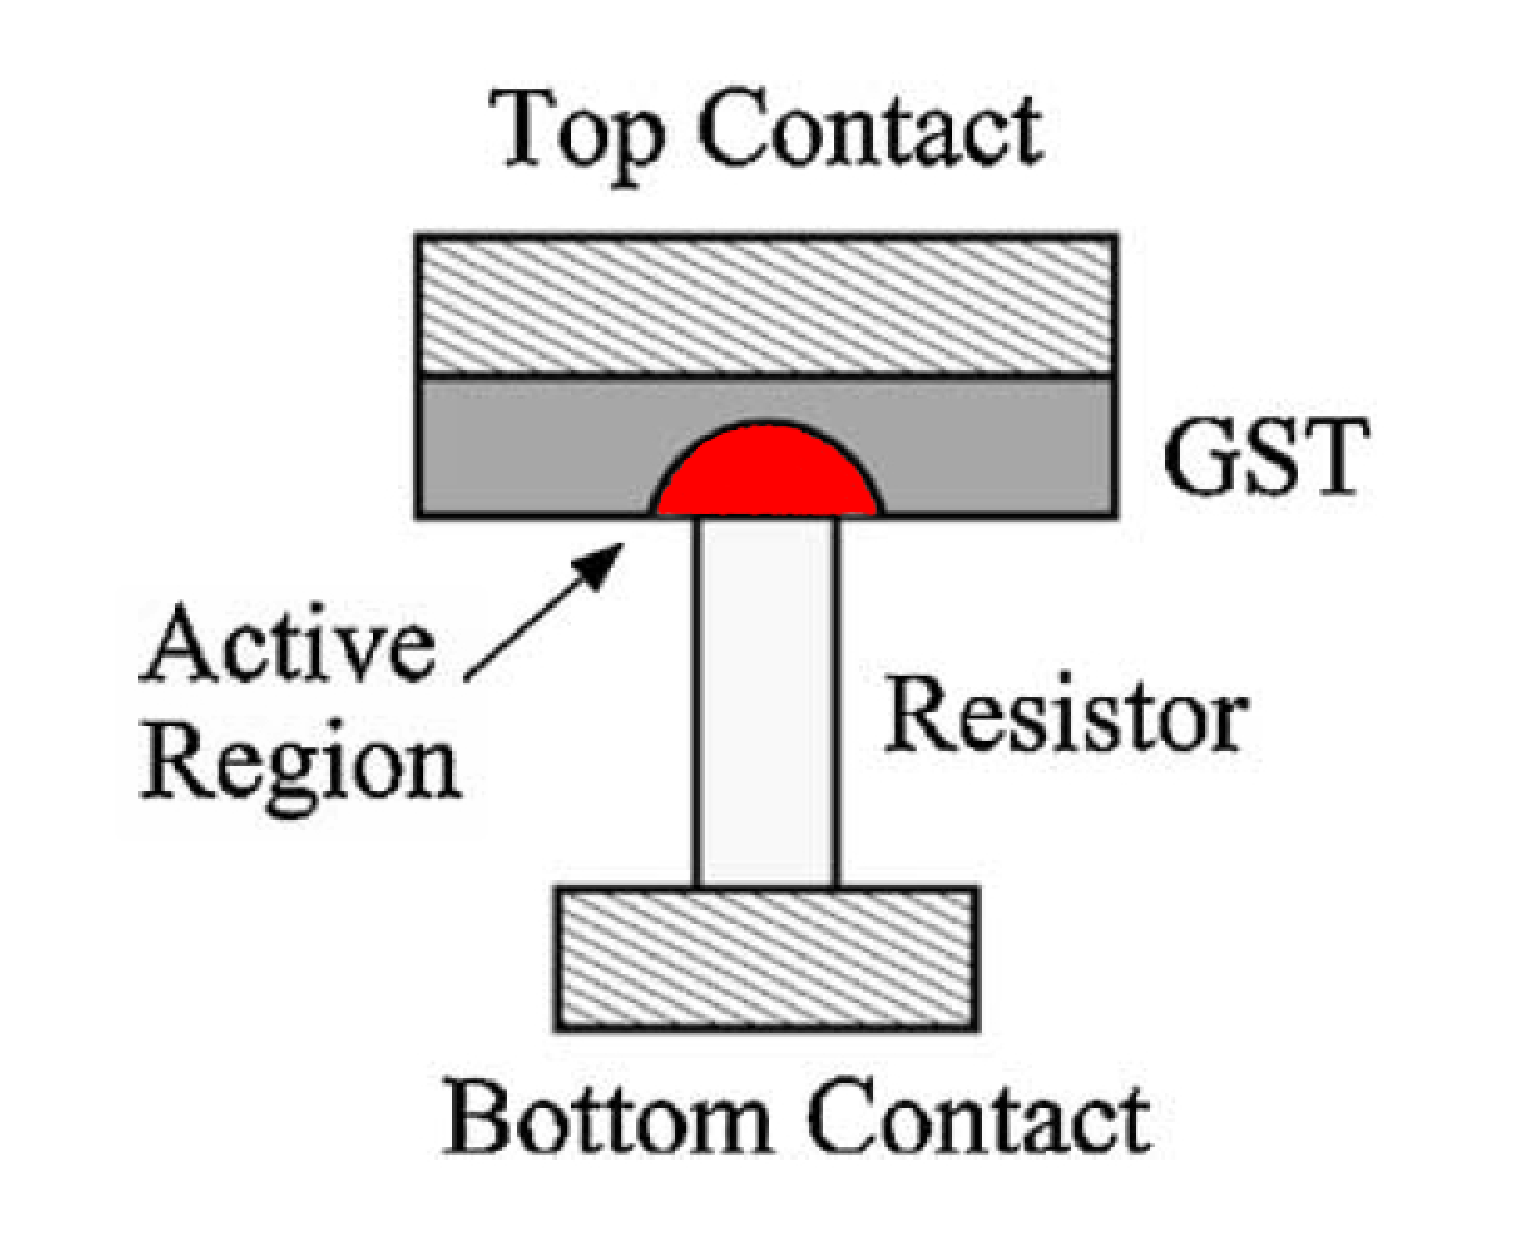
\includegraphics[angle=0, width=0.9\textwidth]{PCMschem.eps}\\
\end{minipage}
\begin{minipage}[c]{0.48\linewidth}
\centering
\includegraphics[angle=0, width=0.9\textwidth]{PCM_SEM.eps}
\end{minipage}
\vspace{2ex}
\begin{minipage}[c]{0.48\linewidth}
\small{
\begin{itemize}
\item Active region: a small drop within GST film undergoes the phase transition\\
\item Phase-change by heating via Joule effect
\end{itemize}
%\begin{center}
%Concept first proposed by\\
%Ovshinsky in 1968
%\end{center}
}
\end{minipage}
\end{frame}

\note{
This is a SEM cross section of a phase change memory and this is a scheme of a PCM cell. 
The PCM cell is formed by a thin film of a phase-change material between a metallic top contact
and a resistor. The active region which undergoes the phase transition is only a small drop of GST
and the transition occurs by heating via Joule effect through the resistor.\\
}

\begin{frame}
\frametitle{I-V characteristic: threshold switching behaviour}
\begin{minipage}[c]{0.58\linewidth}
\begin{itemize}
\item<2-> cell readout: performed at low bias (V $<$ V$_{th}$)
\item<3-> set/reset: bias higher than threshold (V $>$ V$_{th}$)
\end{itemize}
\includegraphics<1>[angle=0, width=1.0\textwidth]{IV1.eps}
\includegraphics<2>[angle=0, width=1.0\textwidth]{IVr.eps}
\includegraphics<3>[angle=0, width=1.0\textwidth]{IVres.eps}
\includegraphics<4>[angle=0, width=1.0\textwidth]{IVs.eps}
\end{minipage}
\begin{minipage}[c]{0.38\linewidth}
\includegraphics<3->[angle=0, width=1.0\textwidth]{pulse.eps}
\begin{itemize}
\item<3-> RESET:\\higher current and shorter pulse
\item<3->[] \ev{crystal {\tiny$\arrowright$} amorphous}
\item<4-> SET:\\lower current and longer pulse
\item<4->[] \ev{amorphous {\tiny$\arrowright$} crystal}
\end{itemize}
\end{minipage}
\end{frame}

\note{
The programming of the PCM cell is possible since phase change materials
show a peculiar current-voltage characteristic. This is the current-voltage characteristic 
of a typical phase change material. The crystal has a ohmic behaviour, while the amorphous phase 
has a high resistivity up to a threshold voltage, then, beyond this threshold, the
system jumps into a highly conductive state which allows Joule heating and recrystallization.
Thus the cell readout is performed at low bias, while the RESET and SET operations are carried out
with bias higher than the threshold. Typically, the threshold voltages are of the order of 1 Volt.
In the RESET operations a high and short current pulse induces the melting of the crystal and the 
amorphous phase is obtained with a rapid quench, while in
the SET operations a lower and longer current pulse induces the crystallization of the amorphous. 
This is the process that control the speed of the device.
}


\begin{frame}
\frametitle{PCM performances}
\begin{center}
\begin{table}[!ht]
\begin{center}
\resizebox*{0.78\textwidth}{!}{
\begin{tabular}{lllll}
\toprule
\rowcolor{themecolor!20!white}
                       & \tbtit{DRAM}    & \tbtit{NOR Flash}     & \tbtit{NAND Flash} & \tbtit{PCM} \\
\bottomrule
\tbtit{Cell Area}      & 6 F$^2$         & 10 F$^2$              & 5 F$^2$            & 16 F$^2$ \\
\midrule
\tbtit{Read Time}      & $<10$ ns        & 10 ns                 & 50 ns              & 60 ns \\
\midrule
\tbtit{Write/Erase}    & $<10$ ns        & $1 \mu$s/10 ms        & 1 ms/0.1 ms        & 50 ns/120 ns \\
\tbtit{Time}           &                 &                       &                    & \\
\midrule
\tbtit{Retention Time} & 64 ms           & $>10$ years           & $>10$ years        & $>10$ years \\
\midrule
\tbtit{Write Cycles}   & $>10^{16}$      & $10^5$                & $10^5$             & $10^9$ \\
\midrule
\tbtit{Write Operating}& 2.5 V           & 12 V                  & 15 V               & 3 V \\
\tbtit{Voltage}        &                 &                       &                    & \\
\midrule
\tbtit{Read Operating} & 1.8 V           & 2 V                   & 2 V                & $<3$ V \\
\tbtit{Voltage}        &                 &                       &                    & \\
\midrule
\tbtit{Multiple-bit}   & No              & In production         & In production      & Research phase \\  
\tbtit{Operation}      &                 &                       &                    & \\
\toprule
\end{tabular}}
\end{center}
\end{table}
\vspace{0.05\textheight}
PCMs show higher speed and better scalability than Flash\\
Goal: Storage Class Memories\\
\end{center}
\end{frame}

\note{
This table compares the performances of PCM and Flash memories. The area of a PCM cell is still 
greater than that of a Flash memory, but PCM cells show a better scalability and higher programming speed than Flash
memories and the endurance is also better with respect to Flash cells. Moreover, the access time is not 
so far from that of DRAM and the future goal is to have memories with speed similar to that of DRAM but 
non-volatile. These are called Storage Class Memories.
}

\begin{frame}
\frametitle{Commercial PCM}
{\ev April 2010} 
\hspace{10em}\raisebox{-1ex}{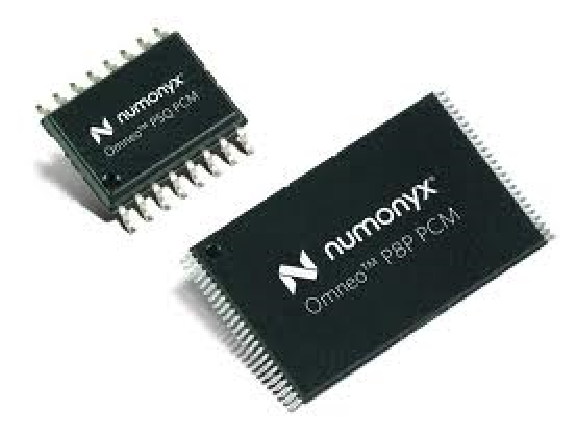
\includegraphics[angle=0, width=0.2\textwidth]{PCM_numonyx.eps}}\\
\vspace{1ex}
\textcolor{themecolor}{Numonyx} (now bought by \textcolor{themecolor}{Micron}) commercialized 
90~nm PCM device\\
Research center based in Agrate Brianza (Milano-Italy)\\
\vspace{3ex}
{\ev July 2012}\\
\vspace{1ex}
\textcolor{themecolor}{Numonyx}: 45~nm devices in production (Agrate)\\
%\vspace{1ex}
\begin{columns}[c]
\column{0.00\textwidth}
\column{0.70\textwidth}
{\ev January 2013}\\
\vspace{1ex}
\textcolor{themecolor}{Nokia} Mobile phone Asha with\\
Micron PCM inside (NOR replacement)\\
\column{0.30\textwidth}
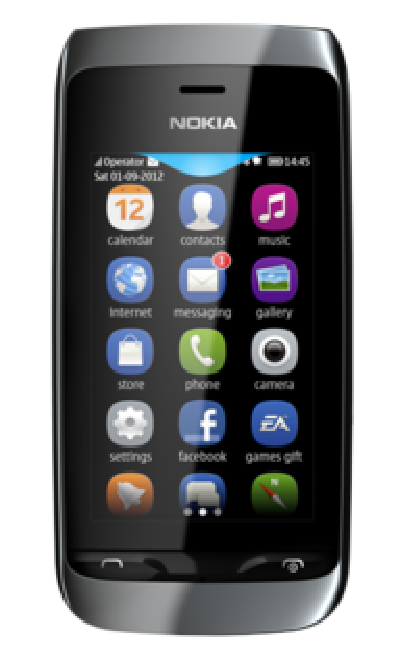
\includegraphics[angle=0, width=0.4\textwidth]{nokia.eps}
\end{columns}
\end{frame}

\note{
These devices are commercial products since 2010 developed by Numonyx now bought by Micron. 
Since 2013, 45nm devices have been used in mobile phones.
}

\begin{frame}
\frametitle{PCM: open issues}
Alloy now employed in PCMs: {\ev Ge$_2$Sb$_2$Te$_5$} (GST)
\vspace{2ex}
\begin{itemize}
\item search for new materials with high crystallization temperature T$_x$ for high temperature 
      automotive applications (125~\celsius)\\
\vspace{2ex}
\item search for materials with lower drift coefficient\\
%\vspace{2ex}
%\item microscopic origin of resistance drift unknown\\
\end{itemize}
\end{frame}

\note{
These devices are commercial, but there is room for improvement.
Now the alloy employed in PCM is the germanium 2 antimony 2 tellurium 5
composition or GST, but the amorphous phase of this compound is not stable 
at high temperatures. Recently new materials with a higher crystallization 
temperature with respect to GST are under scrutiny to improve 
the stability of the amorphous phase for high temperature automotive applications.
Another open issue is resistance drift.
}


%%%%%%%%%%%%%%%%%%%%%%%%%%%%%%%%%%%%%%%%%%%%
%----- Drift ------------------------------%
%%%%%%%%%%%%%%%%%%%%%%%%%%%%%%%%%%%%%%%%%%%%

\begin{frame}
\frametitle{Resistance drift}
\begin{center}
increase of sub-threshold electrical resistance\\
of the amorphous phase with time
\end{center}
\vspace{2ex}
\begin{columns}[c]
\column{0.55\textwidth}
\includegraphics[angle=0, width=1.0\textwidth]{drift_R.eps}
\column{0.45\textwidth}
\begin{center}
\vspace{-5ex}
\begin{displaymath}
R=R_0\left(\frac{t}{t_0}\right)^{\alpha}
\end{displaymath}
$R$ follows a power-law\\
\arrowdown\\
\vspace{1ex}
changes the electrical characteristics of the devices\\
\vspace{6ex}
\end{center}
\end{columns}
\end{frame}

\note{
Drift consists of an increase of the  
electrical resistance of the amorphous phase with time. $R$ increases 
on long time scales of several days by following a power law. This 
phenomenon is detrimental in PCMs since it changes the electrical 
characteristics of the devices.
}

\begin{frame}
\frametitle{Conduction in the amorphous phase}
\vspace{2ex}
\begin{columns}[c]
\column{0.5\textwidth}
\includegraphics[angle=0, width=1.0\textwidth]{a-DOS_arancio.eps}
\column{0.5\textwidth}
\small{
\begin{itemize}
\item valence and conduction bands:\\delocalized states\\
\item Urbach tails\\localized states at band edges\\
\item mobility gap\\energy gap between band edges\\
\end{itemize}
}
\end{columns}
\vspace{2ex}
\small{
\centering
Conduction: thermally activated process, localized states inject holes in vb
\begin{displaymath}
R = R_0 e^{E_A/kT} \qquad  {\textsf{(Poole-Frenkel)}}
\end{displaymath}
\begin{center}
Drift phenomenon due to structural relaxation
\begin{columns}[c]
\column{0.65\textwidth}
\begin{itemize}
\item widening of optical gap from ellipsometry\\
{\tiny 
\cit{[Fantini P. \textit{et al.}, Appl. Phys. Lett. \textbf{100}, 013505 (2012)]}
}
\item modification of in-gap states          
\end{itemize}
\column{0.04\textwidth}
\arrowright
\column{0.31\textwidth}
activation energy $E_A$ for conduction increases, $R$ increases with time \\
\end{columns}
\vspace{2ex}
microscopic origin of structural relaxations unknown
\end{center}
}
\end{frame}

\note{
To understand drift we have to look at the electronic structure of the amorphous phase. 
In an amorphous semiconductor, disorder gives rise to localized states in a mobility 
gap between the valence and the conduction band. States inside the mobility gap 
are localized, while states outside the mobility gap are delocalized. The tails of 
localized states at band edges are the so called Urbach tails.\\
The conduction in the amorphous phase is a thermally activated process where localized 
states inject holes in the valence band. This process is also assisted by an 
external field with a Poole-Frenkel mechanism.\\
Resistance drift is due to structural relaxation of the amorphous which relaxes with 
time in a more stable configuration. The effect of structural relaxations on the 
electronic structure of the amorphous is a widening of the optical gap as revealed by 
ellipsometric measurements and a modification of the in-gap states resulting in an 
increase of the activation energy for conduction and hence of the resistance of the 
amorphous phase.\\
However, the microscopic origin of structural relaxations is unknown.
}

\begin{frame}
\frametitle{Objective}
\centerline{study of more performing PCM materials}
\vspace{3ex}
\begin{itemize}
\item {\ev high T$_x$ materials:} {\it ab-initio} molecular dynamics 
      simulations on InSbTe (InSb as preliminary simulation and In$_3$Sb$_1$Te$_2$) 
      and \\
      GaSbTe (Ga$_4$Sb$_6$Te$_3$) alloys
\vspace{2ex}
\item {\ev drift mechanism:} large scale simulations on GeTe models 
\end{itemize}
\end{frame}

\note{
In this thesis we addressed the two issues we discussed before by performing {\it ab-initio} 
molecular dynamics simulations of InSbTe and GaSbTe alloys. These system have been studied 
experimentally thanks to their high crystallization temperature. In particular we modeled the binary 
InSb as a preliminary simulation and the indium 3 antimony 1 tellurium 2 composition and 
the gallium 4 antimony 6 tellurium 3 composition. Concerning resistance drift, we performed 
large scale simulations on amorphous GeTe aiming at find out a possible drift mechanism. 
}

\section{InSbTe alloys}

\begin{frame}
\frametitle{High T$_x$ alloys: experimental data}
\centering
PCM cells realized with InSbTe and GaSbTe alloys\\
\begin{columns}[c]
\column{0.45\textwidth}
\begin{center}
\includegraphics[angle=0, width=0.8\textwidth]{IST_multilevel.eps}\\
\vspace{-1.5ex}
\hspace{-1.5ex}{\cit{\tiny[E. T. Kim {\it et al.}, \textit{Phys. Status Solidi RRL} \textbf{3}, 103 (2009)]}}
\\
\vspace{1ex}
\includegraphics[angle=0, width=0.8\textwidth]{GaST_perform.eps}\\
\vspace{-1.5ex}
\hspace{-1.5em}{\cit{\tiny[H.-Y. Cheng {\it et al.}, \textit{Appl. Phys. Lett.} \textbf{98}, 121911 (2011)]}}
\\
\end{center}
\column{0.55\textwidth}
\hspace{-1.5em}
\begin{tabular}{ll}
{\ev In$_3$Sb$_1$Te$_2$}:   &{\footnotesize T$_x =$ 292~\celsius\ (T$_m =$ 650~\celsius)}\\
{\ev Ga$_4$Sb$_6$Te$_3$}:   &{\footnotesize T$_x =$ 252~\celsius\ (T$_m =$ 600~\celsius)}\\
{\ev GST}:                  &{\footnotesize T$_x =$ 150~\celsius\ (T$_m =$ 650~\celsius)}\\
\end{tabular}\\
\vspace{3ex}
good of cyclability and stability at high temperature\\
\vspace{3ex}
lack of experimental information on the structure of the amorphous
\end{columns}
\end{frame}

\note{
As regards high crystallization temperature alloys, PCMs cells have already 
been realized with the indium 3 antimony 1 tellurium 2 and the gallium 4 antimony 
6 tellurium 3 which have a higher crystallization temperature with respect to 
GST and a melting temperature that is similar or even lower than that of GST. 
The devices show good ciclability and better thermal stability 
than GST, but a still fast crystallization speed above T$_x$. 
However, no experimental information are available on the structure of the amorphous phases  
which is very important to understand the mechanisms which promote or hider the
crystallization process and control the thermal stability of the amorphous.
}

\begin{frame}
\frametitle{Computational framework}
\begin{itemize}
\item models of the amorphous phase (200-300 atoms) generated by quenching from the
      melt in 100-300~ps from 1000 to 300~K
\vspace{1ex}
\item {\it ab\---initio} (second generation Car\---Parrinello) molecular dynamics simulations\\
      {\cit [T. D. Kühne \textit{et al.}, Phys. Rev. Lett. \textbf{98}, 066401 (2007)]}
\vspace{1ex}
\item density functional theory (DFT), PBE or BLYP exchange and correlation (XC) functional, 
      norm conserving pseudopotentials
\vspace{1ex}
\item Quickstep algorithm, open source CP2K code \\%{\textcolor{bluegreen}{http://cp2k.berlios.de}}\\
      basis set: Gaussian functions (Kohn-Sham orbitals) $+$ plane waves (electronic density)
\end{itemize}
\end{frame}

\note{
In order to analyse the structural features of the amorphous phase of these alloys 
we generated amorphous models by quenching from the melt in hundreds of picoseconds 
from 1000 to 300~K with {\it ab-initio} molecular dynamics simulations. 
In particular, we used a second generation Car-Parrinello method introduced some 
years ago. The ions are treated as classical particles and the trajectories are 
collected by integrating the Newton equations. The forces, instead, are obtained 
by solving the electronic problem for each ionic configuration within the density 
functional theory. We used two different approximations of the exchange and 
correlation functional, the PBE and the BLYP functionals. The acronyms are after the 
name of the authors of the functionals.\\
We explicitly considered only the valence electrons and the interactions with the 
core electrons are described by a pseudopotential. We used the open source CP2K code 
and a particular basis set made of Gaussian functions and plane waves to expand the 
Kohn-Sham orbitals and the electronic density.
}

\begin{frame}
\frametitle{amorphous InSb: structural properties}
\vspace{1ex}
\centering
\begin{columns}[c]
\column{0.4\textwidth}
\centering
Pair correlation functions\\
\vspace{1ex}
\begin{flushright}
\includegraphics[angle=0, width=0.9\textwidth]{ISpbe_tgr.eps}\\
{\cit{\tiny[N. J. Shevchik and W. Paul, \textit{J. Non-Cryst. Solids} \textbf{13}, 55 (1974)]}}\\
\includegraphics[angle=0, width=0.9\textwidth]{ISblyp_tgr.eps}\\
\end{flushright}
\column{0.6\textwidth}
\begin{center}
strong dependence on XC functional\\
\vspace{3ex}
{\ev PBE}\\
overestimation of bond lengths by 5~\%\\
\vspace{2ex}
{\ev BLYP}\\
error on bond lengths $< 1$~\%\\ 
\vspace{3ex}
BLYP better describes structure\\of amorphous InSb
\end{center}
\vspace{3ex}
\end{columns} 
\end{frame}

\note{
We considered first the binary system InSb just to asses the validity of our computational 
framework, in particular the choice of the exchange and correlation functional. 
By averaging on a trajectory at 300~K, we calculated the pair correlation functions of the 
system which give the probability of finding an atom at a distance $r$ from an atom in the 
origin. Here we report the comparison between the experimental pair correlation functions 
and our results obtained with the PBE and the BLYP functionals. We found a strong dependence 
on the exchange and correlation functional, in fact PBE functional gives broader functions 
and overestimates the bond lengths by about 5~\% with respect to the experimental data, 
while the error on bond lengths is less than 1~\% with BLYP functional which better 
describes the amorphous structure of InSb.
}

\begin{frame}
\frametitle{a-InSb: structural properties}
\vspace{1ex}
\centering
{\ev Bond angles distributions}\\
\begin{columns}[t]
\column{0.3\textwidth}
\vspace{1ex}
\begin{itemize}
\setlength{\itemsep}{1.5ex}
\item $90^\circ$ and $180^\circ$:\\
      defective octahedral sites\\
\includegraphics[angle=0,width=0.3\textwidth]{ott3.eps}
\includegraphics[angle=0,width=0.3\textwidth]{ott4.eps}
\includegraphics[angle=0,width=0.3\textwidth]{ott5.eps}\\
      \hspace{-0.5em}\raisebox{1ex}{{\scriptsize (pyramidal)}}\\ 
\item $109.5^\circ$:\\
      tetrahedral sites\\
\includegraphics[angle=0,width=0.3\textwidth]{tetra.eps}\\
\end{itemize}
\column{0.7\textwidth}
\centering
\begin{columns}[c]
\column{0.02\textwidth}
\column{0.4\textwidth}
\vspace{3ex}\\
\centering
\small{
{\ev PBE}\\
tetrahedral atoms\\ 
In: 43~\%\\ 
Sb: 11~\%\\
\vspace{6ex}
{\ev BLYP}\\
tetrahedral atoms\\
In: 68~\%\\
Sb: 52~\%\\
}
\column{0.02\textwidth}
\vspace{3ex}\\
{\scriptsize \arrowright}\\
\vspace{13ex}
{\scriptsize \arrowright}
\column{0.4\textwidth}
\vspace{5ex}\\
mostly octahedral network\\
\vspace{9ex}
mostly tetrahedral network as in 
the crystal (zincblende)
\end{columns}
\end{columns}
\vspace{1ex}
\centerline{BLYP better describes the system}
\end{frame}

\note{
Regarding the geometry of local environments, from the bond angles 
it is possible to distinguish two types of environments: 
defective-octahedral sites with 
bond angles of about 90 and 180 degrees and tetrahedral 
sites with bond angles of about 109 degrees. As shown by the 
bond angles distribution of amorphous InSb, in the PBE model 
there is a predominance of defective-octahedral structures, 
while the BLYP model has a mainly tetrahedral network, closer 
to that of the crystalline phase.\\
So BLYP provides a better description of the system and is 
the exchange and correlation functional we used in the other 
simulations.
}

\begin{frame}
\frametitle{In$_3$Sb$_1$Te$_2$: crystalline structure}
\centerline{Pseudo-binary alloy of InSb and InTe: (InSb)(InTe)$_2$}
\vspace{2ex}
\footnotesize{
\begin{columns}[t]
\column{0.48\textwidth}
\centering
\centerline{{\ev Ternary crystal}}
\begin{center}
Rocksalt phase stable\\between 570 and 470~\celsius
\end{center}
\begin{columns}[c]
\column{0.03\textwidth}
\column{0.27\textwidth}
\centering
\includegraphics[angle=0, width=1.7\textwidth]{c-InSbTep_opt.eps}
\column{0.7\textwidth}
\begin{itemize}
\item cationic sublattice: In 
\item anionic sublattice: randomly occupied by Sb and Te
\item octahedral sites
\end{itemize}
\end{columns}
\vspace{2ex}
\begin{flushleft}
Metastable at 25~\celsius\ by rapidly quenching from the melt
avoiding phase separation in InSb$+$InTe\\
\end{flushleft}
\column{0.04\textwidth}
{ }
\column{0.48\textwidth}
\centering
{\ev Binary crystals}\\
\vspace{2ex}
\begin{columns}[c]
\column{0.4\textwidth}
\centering
\includegraphics[angle=0, width=0.8\textwidth]{c-InSbp.eps}\\
\column{0.6\textwidth}
\textcolor{themecolor}{\bf InSb:} zincblende, tetrahedral environments for In and Sb\\
\end{columns}
\vspace{1ex}
\begin{columns}[c]
\column{0.4\textwidth}
\centering
\hspace{25ex}\includegraphics[angle=0, width=1.1\textwidth]{InTe_tetraedri_z4_glass1.eps}\\
\column{0.6\textwidth}
\textcolor{themecolor}{\bf InTe:} chains of InTe$_4$ edge-sharing tetrahedra\\
\end{columns}
\vspace{1ex}
\begin{flushleft}
\small{
no experimental information on\\the structure of amorphous phase
}
\end{flushleft}
\end{columns}}
\end{frame}

\note{The ternary phase indium 3 antimony 1 tellurium 2 
was then analysed. This composition is a pseudo-binary alloy of the two binary 
InSb and InTe and has a ternary crystalline rocksalt phase stable at high 
temperature with the cationic sublattice occupied by indium atoms and the 
anionic sublattice randomly occupied by antimony and tellurium in octahedral 
sites. This phase can be recovered at room temperature as a metastable phase by rapidly 
quenching from the melt, avoiding phase separation into the two binaries InSb and 
InTe that occurs at low temperature.\\ 
The geometry of the two binary crystals is instead tetrahedral, in particular 
InSb has a zincblende structure, while InTe is formed by chains of edge-sharing 
indium tellurium 4 tetrahedra.\\
At our knowledge, there are no available information on the structure of the amorphous 
phase that is not obvious since there is a competition between the 
octahedral structures of the ternary crystal and the tetrahedral ones of the binaries.
}

\begin{frame}
\frametitle{Ge$_2$Sb$_2$Te$_5$: structure}
\centering
composition used in PCM: pseudo-binary alloy (GeTe)$_2$(Sb$_2$Te$_3$)$_1$\\
\vspace{4ex}
\begin{columns}[t]
\column{0.5\textwidth}
\centering
{\ev Ternary crystal}\\
cubic rocksalt\\ 
octahedral-like environments\\
\vspace{2ex}
{\ev Binary crystals}\\
\begin{description}
\item[GeTe:] cubic rocksalt\\octahedral sites\\
\item[Sb$_2$Te$_3$:] rhombohedral lamellar structure\\
octahedral sites
\end{description}
\column{0.5\textwidth}
\centering
{\ev Amorphous GST/GeTe}\\
mainly octahedral-like network\\ 
\includegraphics[angle=0,width=0.2\textwidth]{ott3.eps}
\includegraphics[angle=0,width=0.2\textwidth]{ott4.eps}
\includegraphics[angle=0,width=0.2\textwidth]{ott5.eps}\\
with a minority fraction of tetrahedral Ge ($\sim30$~\%)\\ 
\includegraphics[angle=0,width=0.2\textwidth]{tetra.eps}\\
{\cit\tiny{[S. Caravati {\it et al.}, \textit{Appl. Phys. Lett.} \textbf{91}, 171906 (2007)]}}
\end{columns}
\end{frame}

\note{
For GST, instead, the ternary and the two binary crystals, germanium telluride and
antimony 2 tellurium 3 of which GST is made of, have an octahedral network. In this 
case the structure of the amorphous is mostly octahedral-like as the crystals, but with 
a minority fraction of tetrahedral germanium atoms. The structure of amorphous GeTe is 
very similar with a predominance of octahedral structures.
}

\begin{frame}
\frametitle{a-In$_3$Sb$_1$Te$_2$: structural properties}
\begin{columns}[c]
\column{0.38\textwidth}
\centering
Pair correlation functions\\
\vspace{2ex}
\includegraphics[angle=0, width=1.0\textwidth]{ISTblyp_gr.eps}
\column{0.58\textwidth}
\centering
Coordination numbers
\only<1>{\begin{table}[!ht]
\begin{center}
\resizebox*{0.78\textwidth}{!}{
\begin{tabular}{ccccc}
\toprule
\rowcolor{themecolor!20!white}
              & \tbtit{with In} & \tbtit{with Sb} & \tbtit{with Te} & \tbtit{tot} \\
\bottomrule
\tbtit{In}    & 0.95         & 0.78         & 1.93         & 3.66           \\
\midrule
\tbtit{Sb}    & 2.35         & 0.92         & 0.28         & 3.55           \\
\midrule
\tbtit{Te}    & 2.89         & 0.14         & 0.00         & 3.04           \\ 
\toprule
\end{tabular}}
\end{center}
\end{table}}
\centering
\only<1>{very few Sb-Te bonds\\{\footnotesize\arrowdown}\\
\vspace{1ex}
solid solution of InSb and InTe}
\only<2>{
\vspace{2ex}\\
\begin{columns}[c]
\column{0.58\textwidth}
\includegraphics<2>[angle=0,width=1.0\textwidth]{ISTblyp_nc.eps}
\column{0.38\textwidth}
\centering
very few Sb-Te bonds\\{\footnotesize\arrowdown}\\
\vspace{1ex}
solid solution of InSb and InTe         
\end{columns}}
\end{columns}
\end{frame}

\note{
These are the pair correlation functions of the amorphous and these the 
coordination numbers obtained by integrating the pair correlation functions.
Very few Sb-Te bonds are present in the structure while there is high 
fraction of In-Sb and In-Te bonds. So the amorphous appears as a solid 
solution of InSb InTe. From the coordination numbers distributions, indium 
and antimony are both mostly four-fold coordinated as in InSb, 
while Te is three-fold coordinated.
}

\begin{frame}
\frametitle{a-In$_3$Sb$_1$Te$_2$: structural properties}
\centering
Bond angles distributions\\
\vspace{3ex}
\begin{columns}[c]
\column{0.02\textwidth}
{ }
\column{0.5\textwidth}
\includegraphics[angle=0,width=1.0\textwidth]{ISTblyp_tpteta.eps}
\column{0.48\textwidth}
\centering
$\sim109^\circ$ bond angles: \\
\centering
mainly tetrahedral network\\
\vspace{2ex}
\begin{itemize}
\setlength{\itemsep}{1.5ex}
\item tetrahedral In: 77~\%\\(16~\% edge-sharing)\\
\item tetrahedral Sb: 45~\%\\
\item pyramidal Te
\raisebox{-2ex}{\includegraphics[angle=0,width=0.2\textwidth]{ott3.eps}}
\end{itemize}
\end{columns}                      
\end{frame}

\note{
The bond angles distributions of indium and antimony are piked at 
about 109 degrees resulting in a mainly tetrahedral 
network. In particular, the 77~\% of indium atoms  
are tetrahedral and among them the 16~\% forms 
edge-sharing tetrahedra as in crystalline InTe. 
Almost one half of antimony atoms is also tetrahedral, 
while three-fold coordinated Te atoms have a pyramidal 
environment.
}

\section{GaSbTe alloys}

\begin{frame}
\frametitle{Ga$_4$Sb$_6$Te$_3$: crystalline structure}
\centerline{Pseudo-binary alloy of GaSb and Sb$_2$Te$_3$: (GaSb)$_4$(Sb$_2$Te$_3$)$_1$}
\vspace{1ex}
\small{
\begin{columns}[t]
\column{0.5\textwidth}
\begin{columns}[c]
\column{0.05\textwidth}
\column{0.45\textwidth}
\includegraphics[angle=0,width=1.0\textwidth]{GaSb.eps}\\
\vspace{2ex}
\includegraphics[angle=0,width=1.0\textwidth]{Sb2Te3.eps}\\
\column{0.5\textwidth}
{\ev GaSb:}
zincblende sructure with 
tetrahedral sites for Ga and Sb\\
\vspace{6ex}
{\ev Sb$_2$Te$_3$:}
rhombohedral lamellar structure 
with octahedral environments\\
\end{columns}
\column{0.5\textwidth}
\begin{columns}[c]
\column{0.05\textwidth}
\column{0.4\textwidth}
\includegraphics[angle=0,width=1.0\textwidth]{GaTev.eps}\\
\column{0.45\textwidth}
{\ev GaTe:}
monoclinic lamellar structure
with tetrahedral Ga and Ga-Ga dimers\\
\end{columns}
\end{columns}
}
\vspace{2ex}
\begin{center}
Rhombohedral crystalline structure Ga$_4$Sb$_6$Te$_3$\\ 
expected octahedral environments as in GST
\end{center}
\end{frame}

\note{
The other high crystallization temperature alloy we analysed is 
the gallium 4 antimony 6 tellurium 3 composition which is a 
pseudo-binary alloy of GaSb and antimony 2 tellurium 3. 
In this case the two binary crystals have very different structures: 
GaSb has a zincblende structure with tetrahedral environments, while 
antimony 2 tellurium 3 has a rhombohedral lamellar structure with 
six-fold coordinated antimony in octahedral environments.\\ 
The other binary crystal relevant for GaSbTe alloys is GaTe 
which has a monoclinic lamellar structure with tetrahedral Ga atoms 
and dimers of gallium.\\
The strucure of the ternary crystal has not been fully resolved yet, 
but it is rhombohedral with probably octahedral environments as in 
crystalline GST.
}

 
\begin{frame}
\frametitle{a-Ga$_4$Sb$_6$Te$_3$: structural properties}
\centerline{Pair correlation functions and coordination numbers}
\centerline{of a melt-quenched 299-atom amorphous model}
\begin{columns}[c]
\column{0.38\textwidth}
\vspace{2ex}
\includegraphics[angle=0, width=1.0\textwidth]{GaST_gr.eps}
\column{0.58\textwidth}
\begin{table}[!ht]
\begin{center}
\resizebox*{0.78\textwidth}{!}{
\begin{tabular}{ccccc}
\toprule
\rowcolor{themecolor!20!white}
              & \tbtit{with Ga} & \tbtit{with Sb} & \tbtit{with Te} & \tbtit{tot} \\
\bottomrule
\tbtit{Ga}    & 0.37    & 1.76    & 1.67    & 3.80                          \\
\midrule
\tbtit{Sb}    & 1.16    & 1.89    & 0.19    & 3.25                          \\
\midrule
\tbtit{Te}    & 2.23    & 0.38    & 0.00    & 2.61                          \\
\toprule
\end{tabular}}
\end{center}
\end{table}
\begin{itemize}
\item very few Sb-Te bonds:\\
      solid solution of GaSb and GaTe\\
\item high fraction of Ga-Ga bonds:\\
      Ga-Ga dimers as in c-GaTe\\
\item tetrahedral network as c-GaSb and c-GaTe\\
\item high fraction of Sb-Sb bonds:\\
      segregation of Sb 
\end{itemize}
\end{columns}
\end{frame}

\note{
Pair correlation functions and partial coordination numbers were 
calculated for a melt quenched amorphous model that, as already 
found for indium 3 antimony 1 tellurium 2, shows very few Sb-Te 
bonds and can be seen as a solid solution of GaSb and GaTe. 
Moreover, a not negligible fraction of homopolar Ga-Ga bonds 
are present as in the GeTe crystal and the network is mainly 
tetrahedral as in crystalline GaSb and GaTe. The model presents 
also a sizable fraction of Sb-Sb homopolar bonds as a result of 
the partial segregation of antimony.
}

\begin{frame}
\frametitle{a-Ga$_4$Sb$_6$Te$_3$: structural properties}
\centerline{Segregation of antimony}
\vspace{1ex}
\begin{columns}[c]
\column{0.1\textwidth}
\column{0.5\textwidth}
\includegraphics[angle=0, width=1.0\textwidth]{GaST_sbcluster.eps}
\column{0.5\textwidth}
\includegraphics[angle=0, width=0.75\textwidth]{GaST_cluster.eps}
\end{columns}
\begin{itemize}
\item only 4~\% of Sb atoms with only heteropolar bonds\\
\item dimers and chains 4-, 5- and 6-atoms long\\
\item two clusters of 13 and 97 Sb atoms\\
\end{itemize}
\end{frame}

\note{
In fact, we found that only 4~\% of Sb atoms form only heteropolar 
bonds, while dimers and small chains of antimony atoms are present. 
Most of the antimony atoms form a 13- and a 97-atom clusters, 
the shape of the biggest one is represented in this picture.
So there is a partial segregation of antimony.
}

\begin{frame}
\frametitle{High T$_x$ alloys: conclusions}
\begin{enumerate}
\item prevalence of In-Sb and In-Te bonds in a-In$_3$Sb$_1$Te$_2$ and of Ga-Sb and Ga-Te bonds 
      in a-Ga$_4$Sb$_6$Te$_3$, very few Sb-Te bonds: ternary alloys as mixture of InSb-InTe and 
      GaSb-GaTe binary compounds
\vspace{2ex}
\item mainly tetrahedral networks as in binary crystals InSb, InTe and GaSb, GaTe 
\vspace{2ex}
\item tetrahedral structures absent in the octahedral ternary crystals hinder the crystallization
\end{enumerate}
\end{frame}

\note{
In conclusion, our simulations on high crystallization temperature InSbTe and GaSbTe alloys 
have reported a prevalence of In-Sb and In-Te bonds in a-In$_3$Sb$_1$Te$_2$ and of Ga-Sb and 
Ga-Te bonds in a-Ga$_4$Sb$_6$Te$_3$ together with very few Sb-Te bonds. Thus the ternary alloys 
can be thought as mixtures of InSb-InTe and GaSb-GaTe.\\
As opposed to amorphous GST, the two alloys have mainly tetrahedral network as the binary crystals 
and the presence of tetrahedral structures that are absent in the octahedral ternary crystals 
probably hinders the crystallization process resulting in a higher crystallization temperature 
with respect to GST.
}

\section{GeTe}

\begin{frame}
\frametitle{Atomistic simulations of resistance drift}
\begin{itemize}
\addtolength{\itemindent}{2em}
\item search for new materials with low drift coefficients
\item lack of a microscopic understanding of resistance drift
\end{itemize}
\vspace{4ex}
\centering
\begin{columns}[c]
\column{0.05\textwidth}
\column{0.35\textwidth}
drift depends on in-gap defect states
\column{0.05\textwidth}
{\small\arrowright}
\column{0.55\textwidth}
need to simulate large systems\\($10^3$ atoms), beyond the reach of 
{\it ab-initio} molecular dynamics {\scriptsize\arrowright}\\ 
\vspace{2ex}
classical molecular dynamics simulations with Neural Network potential
\end{columns}
\end{frame}

\note{
As a second topic, we addressed the study of drift in the amorphous.
In order to increase the stability of PCM cells, new materials with low drift 
coefficients are needed. However, a microscopic understanding of this phenomenon 
still lacks. To address this issue we thus performed atomistic simulations on 
large models of amorphous GeTe. Resistance drift depends on the in-gap states. 
So, in order to study this phenomenon, we need a good statistics on the in-gap states, 
so large models of thousands of atoms. However, such large systems are beyond the 
reach of {\it ab-initio} molecular dynamics, so we performed classical molecular 
dynamics simulations with a neural network potential built on a huge {\it ab-initio}
database.
}

\begin{frame}
\frametitle{Neural Network potential}
\centering
Total energy as a sum of the atomic energies: $E_{tot} = \sum_i E_i$
\begin{flushright}
{\cit{[Behler J. and Parrinello M., Phys. Rev. Lett. 2007]}}
\end{flushright}
\vspace{3ex}
\begin{columns}[c]
\column{0.50\textwidth}
\begin{displaymath}
E_i = F(\{G(\bar{x})\}) 
\end{displaymath}
\column{0.50\textwidth}
\centering
{\ev{Symmetry functions $\{G\}$}}\\
Information on the atomic environment
up to a certain cut-off radius
(3$^{rd}$ coordination shell)\\
\end{columns}
\vspace{2ex}
\begin{columns}[c]
\column{0.50\textwidth}
\centering
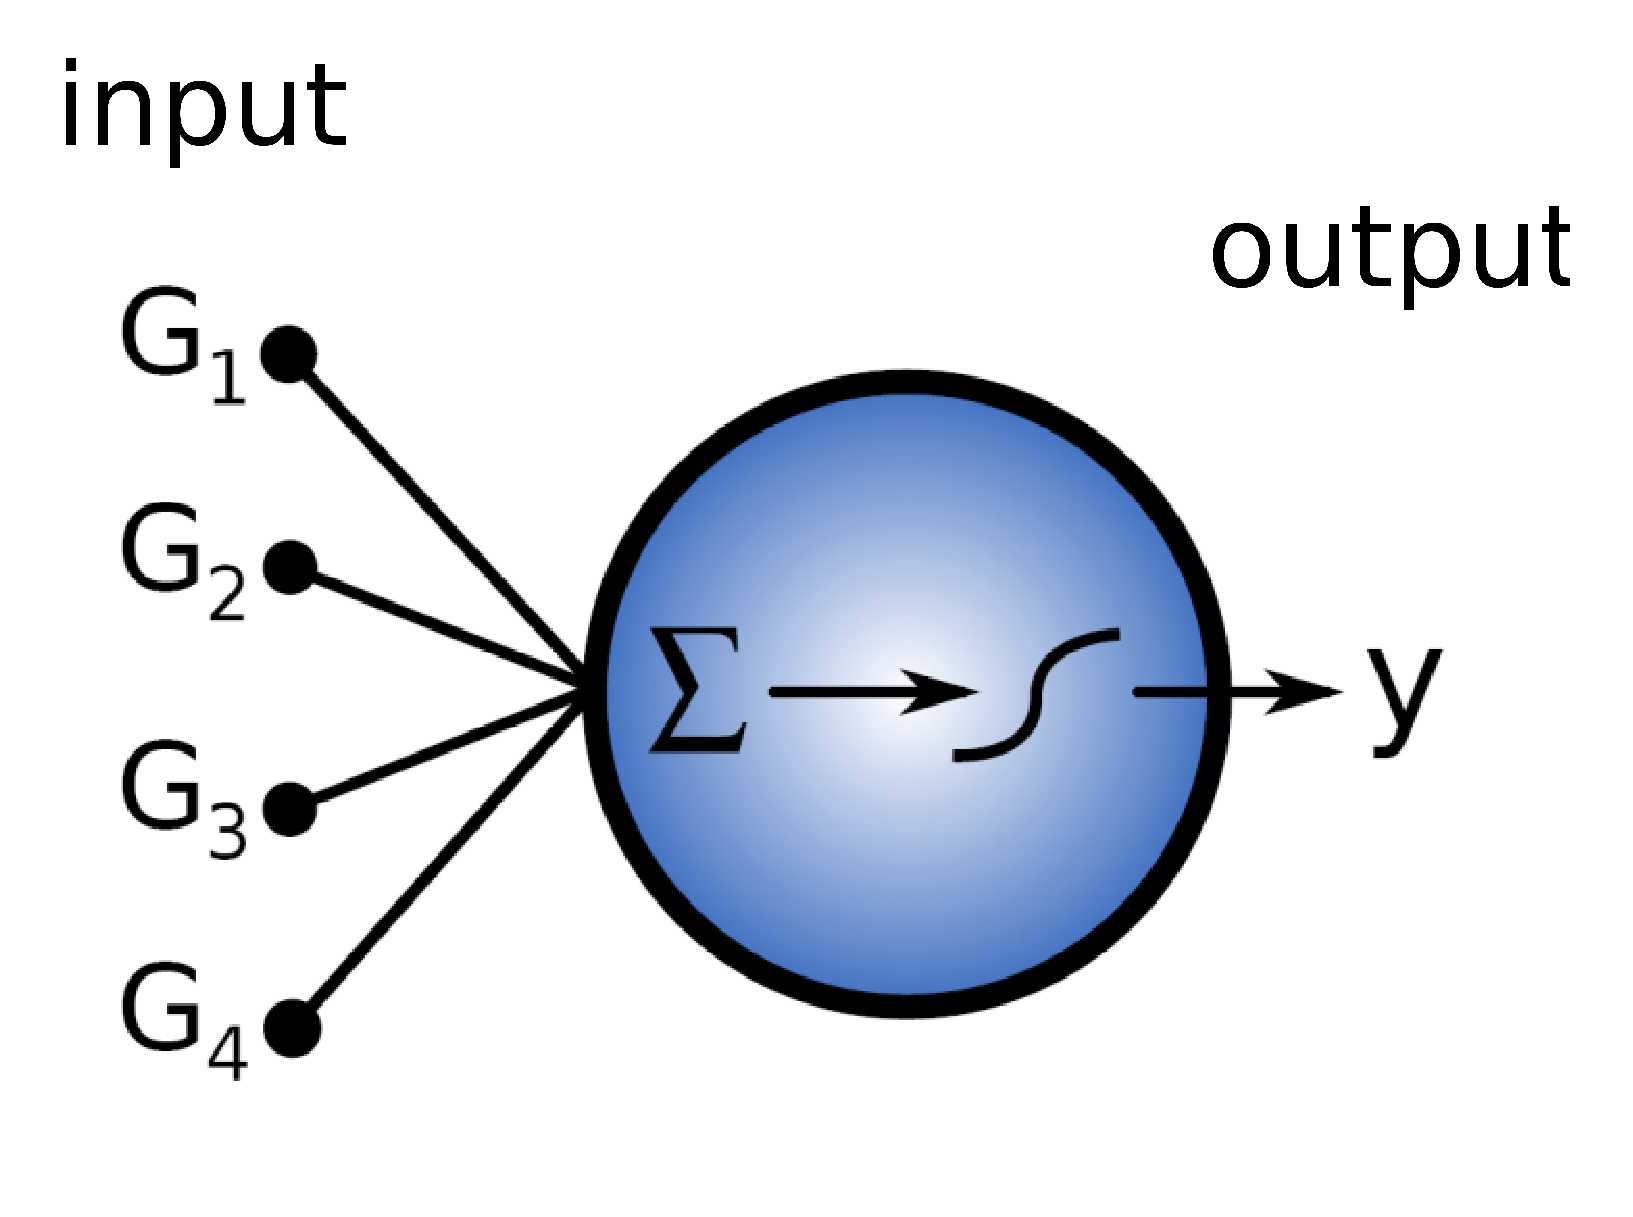
\includegraphics[angle=0, width=0.7\textwidth]{NN_schema.eps}
\column{0.50\textwidth}
$E_i$ analytic function of the atomic positions
\end{columns}
\end{frame}

\note{
The neural network potential is built by writing the total energy as 
a sum of the atomic energies which depend on the atomic local environment. 
And the local environment is described by the symmetry functions $G$ 
which depend on bond lengths and bond angles up to a certain cut-off distance 
that in our case include the third coordination shell.\\
The neural network is a scheme to assign an energy to a single atom given the 
local environment. The atomic energy is an analytic function of the atomic 
positions, so it is easy to calculate forces. 
}

\begin{frame}
\frametitle{Neural Network potential for GeTe}
\begin{columns}[c]
\column{0.55\textwidth}
\centering
$E_i$ calculated through a neural network\\
\vspace{4ex}
\resizebox*{0.9\textwidth}{!}{
\begin{tikzpicture}
  %%Create a style for the arrows we are using
  \tikzset{normal arrow/.style={draw,-stealth',very thick,color=themecolor}}
  \tikzset{little arrow/.style={draw,-stealth',thick,color=themecolor!60!white}}
  \tikzset{node circle/.style={circle,shading=ball,ball color=themecolor,text=white}}
  \tikzstyle{layer} = [text width=4em, text centered]
  %%Create the different coordinates to place the nodes
  \path (0,0) coordinate (g1) ++(0,-2.5) coordinate (g2); %++(0,-2) coordinate (3);
  \path (g1) ++(-1.3,-.5) coordinate (x1);
  \path (g2) ++(-1.3,+.5) coordinate (x2);
  %%Use the calc library and partway modifiers to generate the second and third level points
  \path ($(g1)!.5!(g2)!2.2 cm!90:(g2)$) coordinate (y2);
  \path (y2) ++(0,2) coordinate (y1);
  \path (y2) ++(0,-2) coordinate (y3);
  \path (y2) ++(1.7,0) coordinate (e);
  %%Place nodes at each point using the foreach construct
  \foreach \in/\i/\color in {g1/1/themecolor!60,g2/2/themecolor!60}{
%    \node[draw,circle,shading=axis,top color=\color, bottom color=\color!black,text=white,shading angle=45] (n\in) at (\in) {$G_{\i}$};
    \node[node circle] (n\in) at (\in) {$G_{\i}$};
  }
  \foreach \in/\i/\color in {y1/1/themecolor!60,y2/2/themecolor!60,y3/3/themecolor!60}{
%    \node[draw,circle,shading=axis,top color=\color, bottom color=\color!black,text=white,shading angle=45] (n\in) at (\in) {$y_{\i}$} 
%         node[above of =n\in,node distance=2em]{$f_{\i}$};
    \node[node circle] (n\in) at (\in) {$y_{\i}$} node[above of =n\in,node distance=2em]{$f_{\i}$};
  }
%  \node[draw,circle,shading=axis,top color=themecolor!60, bottom color=themecolor!60!black,text=white,shading angle=45] (ne) at (e) {$\;\;E_{i}\;\;$}; 
  \node[node circle] (ne) at (e) {$\;\;E_{i}\;\;$};
  %%Place the remaining nodes separately
  \node (nx1) at (x1) {$\mathbf{x_1}$};
  \node (nx2) at (x2) {$\mathbf{x_2}$};
  %%Layer titles
  \node[layer,above of=ny2, node distance=22ex] (hl) {Hidden layer};
  \node[layer,left of=hl, node distance=2.2cm] (il) {Input layer};
  \node[layer,above of=e, node distance=22ex] (ol) {Output layer};
  %%Drawing the arrows
  \path[little arrow] (nx1) -- (ng1);
  \path[little arrow] (nx1) -- (ng2);
  \path[little arrow] (nx2) -- (ng1);
  \path[little arrow] (nx2) -- (ng2);
  \path[normal arrow] (ng1) -- node[above=.0em,Black] {$a_{11}^{01}$} (ny1);
  \path[normal arrow] (ng1) -- node[above=.0em,Black] {$a_{12}^{01}$} (ny2);
  \path[normal arrow] (ng1) -- node[below=-2.0em,left=1.4em,Black] {$a_{13}^{01}$} (ny3);
  \path[normal arrow] (ng2) -- (ny1);
  \path[normal arrow] (ng2) -- (ny2);
  \path[normal arrow] (ng2) -- node[below=0.0em,Black] {$a_{23}^{01}$} (ny3);
  \path[normal arrow] (ny1) -- node[above=0.2em,Black] {$a_{11}^{12}$} (ne);
  \path[normal arrow] (ny2) -- node[above=0.1em,Black] {$a_{21}^{12}$} (ne);
  \path[normal arrow] (ny3) -- node[above=0.5em,Black] {$a_{31}^{12}$} (ne);
\end{tikzpicture}}
\column{0.45\textwidth}
\vspace{2ex}
\small{
\mbox{$E_i = \sum_{j=1}^3{a_{j1}^{12}\cdot f\left(\sum_{k=1}^2{G_k\cdot a_{kj}^{01}}\right)}$}\\
}
\vspace{2ex}
\centering\includegraphics[angle=0, width=0.7\textwidth]{NNhtan.eps}\\
\vspace{3ex}
neural network potential for GeTe:\\
\begin{itemize}
\item 8000 fitting parameters
\item $30 000$ configurations
\end{itemize}
\end{columns}
\end{frame}

\note{
This picture represent a simple scheme of a neural network.
The symmetry functions are obtained from the atomic positions and are the input 
values of the network. We take a linear combination of the symmetry functions with 
these weights $a$ to obtain these intermediate values $y$. Then we apply a non linear 
function $f$ with this form to the $y$s and the results are again linearly combined to 
obtain the atomic energy. The weights $a$ are the fitting parameters of the potential. 
In our case for GeTe the network has 8 thousand parameters fitted on 30 thousand 
configurations.  
}


\begin{frame}
\frametitle{Neural Network potential for GeTe}
\centering
Pair correlation functions of a-GeTe at 300~K
\begin{columns}[c]
\column{0.55\textwidth}
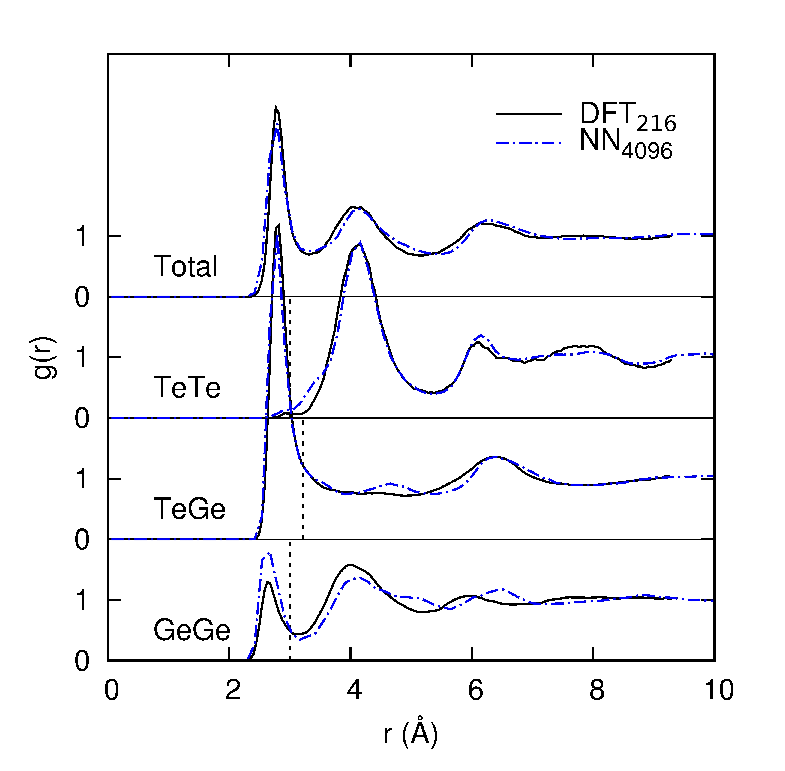
\includegraphics[angle=0, width=1.1\textwidth]{GT_grNN_DFT.eps}
\column{0.40\textwidth}
Neural Network potential describes well amorphous/liquid phase of GeTe\\
\vspace{2ex}
\begin{flushright}
\cit{[Sosso G. C. {\it et al.}, Phys. Rev. B {\bf 85}, 174103 (2012)]}
\end{flushright}
\end{columns}
\end{frame}

\note{
The Neural Network potential for GeTe developed in our group reproduces well the structure of 
amorphous, crystalline and liquid GeTe, in particular the comparison between pair correlation functions 
calculated on an {\it ab-initio} 216-atom model and on a neural network 4 thousand-atom 
model shows a very good agreement. 
}

\begin{frame}
\frametitle{Models of a-GeTe}
\begin{itemize}
\item several models of amorphous GeTe (1728 atoms) generated by quenching from the melt (1000-300~K) 
      in 100~ps\\
\vspace{1ex} 
\item classical molecular dynamics simulations with Neural Network potential %and DL-POLY $+$ RuNNer code\\
\vspace{1ex}
\item {\it ab-initio} (PBE) relaxation of amorphous models %with the CP2K code 
\vspace{1ex}
\item electronic structure calculated at the DFT level %with Engel-Vosko functional 
\end{itemize}
\end{frame}

\note{
To study the drift we generated several models of amorphous GeTe of about 2000 atoms by 
quenching the melt from 1000 to 300~K in 100~ps with classical molecular dynamics simulations 
and the neural network potential. The amorphous models were then relaxed by first principles 
with the PBE functional and the electronic structure was computed at the DFT level.
}

\begin{frame}
\frametitle{a-GeTe: electronic properties}
\centerline{in-gap localized states}
\vspace{4ex}
\begin{columns}[c]
\column{0.01\textwidth}
\column{0.55\textwidth}
\centering
{\scriptsize
Inverse Participation Ratio\\
measure of the localization of each state\\
}
\vspace{2ex}
\includegraphics[angle=0, width=1.0\textwidth]{GT_dosipr.eps}
\column{0.36\textwidth}
\centering
Defect states in band gap and near vb edge localized on
chains of Ge-Ge bonds\\
\includegraphics[angle=0, width=0.6\textwidth]{chain32at_tesi.eps}
\column{0.03\textwidth}
\end{columns}
\end{frame}

\note{
For each amorphous model we computed the electronic density of states 
and the Inverse Participation Ratio which is a measure of the localization 
of each state. The models present several defect states in the band gap 
and near the valence band edge which are localized on chains of Ge atoms.
}

\begin{frame}
\frametitle{Drifted a-GeTe models}
\centering
annealing at 500~K to mimic drift\\
\vspace{2ex}
\begin{columns}[c]
\column{0.6\textwidth}
\centering
\includegraphics[angle=0, width=0.9\textwidth]{GT_dosipr_ann.eps}
\column{0.4\textwidth}
\begin{itemize}
\item reduction of Ge-Ge chains
\item reduction of in-gap states
\item increase of the localization 
\item widening of band gap
\end{itemize}
\end{columns}
\end{frame}

\note{
To mimic the drift which occurs at room temperature on long time scales, the 
we annealed the models at high temperature and we see a reduction of the 
chains of Ge-Ge bonds, a reduction of the in-gap states due to the removal 
of a part of the chains and an increase of the localization due to the shortening 
of the chains. As a consequence of the decrease of the number of defect states, 
the band gap increases. However this is obtained at high temperature where other 
transformations may occur. To mimic drift at room temperature, we used a computational 
technique called metadynamics to accelerate the structural transformation.
}

 

\begin{frame}
\frametitle{Metadynamics}
\centering
Study of rare events\\ 
\vspace{4ex}
\begin{columns}[c]
\column{0.5\textwidth}
\includegraphics<1>[angle=0, width=1.0\textwidth]{meta0.eps}
\includegraphics<2>[angle=0, width=1.0\textwidth]{meta1.eps}
\includegraphics<3>[angle=0, width=1.0\textwidth]{meta2.eps}
\includegraphics<4>[angle=0, width=1.0\textwidth]{meta3.eps}
\includegraphics<5>[angle=0, width=1.0\textwidth]{meta4.eps}
\includegraphics<6>[angle=0, width=1.0\textwidth]{meta5.eps}
\includegraphics<7>[angle=0, width=1.0\textwidth]{meta6.eps}
\column{0.5\textwidth}
\begin{itemize}
\item reaction coordinate described by collective variables, 
      functions of atomic positions\\
      $s=s(\{{\mathbf R}\})$
\item external biasing potential in the space of $s$ 
      sum of Gaussian functions 
      induces the structural transformation
\end{itemize}
\begin{flushright}
{\cit{[A. Laio and M. Parrinello, Proc. Nat. Acad. Sci. \textbf{99}, 12562 (2002).]}}
\end{flushright}
\end{columns}
\end{frame}

\note{
Metadynamics is typically used to study rare events and 
phenomena that occur on long time scales.
In this method we define reaction coordinates called collective 
variables which depend on the atomic position and are able to discriminate 
between the initial and the final state of the transformation. The 
collective variables are typically geometrical parameters.
During the dynamics an external biasing potential sum of Gaussian functions 
is added to the Hamiltonian of the system to induce the structural 
transformation. The Gaussian functions added during the simulations fill 
the potential well forcing the system to visit other minima in the free 
energy surface.
}


\begin{frame}
\frametitle{a-GeTe: metadynamics simulations}
\vspace{1ex}
\begin{columns}[c]
\column{0.6\textwidth}
\includegraphics[angle=0, width=0.9\textwidth]{GT_dosipr_meta.eps}
\column{0.4\textwidth}
collective variables: Ge-Ge and Ge-Te coordination numbers\\
\vspace{2ex}
\centering
After metadynamics:
\vspace{1ex}
\begin{itemize}
\item energy gain, smaller number of Ge-Ge chains
\item decrease in number of in-gap states
\item increase of localization
\item widening of band gap
\end{itemize}
\end{columns}
\end{frame}

\note{
In our case, since we want to reduce the number of Ge-Ge bonds 
and increase the number of Ge-Te bonds, we chose as collective 
variables the partial coordination numbers of germanium with Ge atoms 
and with Te atoms.\\ 
After a metadynamics run at 300~K and an {\it ab-initio} relaxation, 
we obtained a model which is more stable than the starting 
configuration and with a smaller number of homopolar Ge-Ge bonds.
As a consequence of the reduction of the Ge-Ge chains, the number 
of in-gap states decreases, while the band gap increases.
We can propose that drift originates from removal of chains of Ge-Ge 
bonds with time.
}

\begin{frame}
\frametitle{Drift in a-GeTe: conclusion}
{\large
\centering
structural relaxations towards a more stable amorphous\\
\vspace{2ex}
removal of Ge-Ge chains leads to 
\vspace{2ex}
\begin{itemize}
\addtolength{\itemindent}{6em}
\item decrease in number of in-gap states
\item widening of band gap
\end{itemize}
\vspace{1ex}
\arrowdown\\
\vspace{2ex}
\centerline{\Large resistance drift}
\vspace{3ex}
Ge-Ge chains responsible also for high crystallization speed
}
\end{frame}

\note{
We can conclude that structural relaxations in the amorphous phase consist of removal of 
chains of Ge-Ge bonds which leads to a decrease of the number of 
in-gap states and to an increase of the band gap which can account 
for resistance drift.\\
The presence of chains of Ge-Ge bonds is responsible also for the high crystallization 
speed of GeTe.
}

\begin{frame}
\frametitle{Origin of fast crystallization}
{\ev Structural heterogeneities} (Ge-Ge chains) \qquad\arrowright 
\vspace{1.5ex}
\begin{itemize}
\addtolength{\itemindent}{4em}
\setlength{\itemsep}{1.5ex}
\item dynamical heterogeneities in the supercooled liquid
\item breakdown of Stokes-Einstein relation: {\large $D\xcancel{\propto} T/\eta$}
\item fragility
\raisebox{-10ex}{\includegraphics[angle=0, width=0.35\textwidth]{fragility.eps}}
\end{itemize}
\centering
\vspace{1.5ex}
high mobility at high supercooling \quad{\scriptsize\arrowright}\quad%\\
high crystal growth velocity
\end{frame} 

\note{
In fact, simulations on supercooled liquid GeTe carried out in our group 
have shown the presence of structural heterogeneities in the form of Ge chains 
that give rise to dynamical heterogeneities. Dynamical heterogeneities consist of 
regions where atoms move faster and regions where atoms move slower spatially separated.
Dynamical heterogeneities are responsible for the breakdown of the Stokes-Einstein 
relation between the self-diffusion coefficient $D$ and the viscosity $\eta$ which 
is a typical feature of fragile liquids. In a fragile liquid, the viscosity remains 
low down to temperatures close to the glass transition temperature and then there 
is a steep raise of $\eta$ to reach the value expected at T glass. While for a 
strong liquid the viscosity has an Arrhenius behaviour. 
Both the breakdown of the Stokes-Einstein relation and the fragility result in a 
high atomic mobility which is the ultimate source of the high crystal growth velocity.
}


\begin{frame}
\frametitle{Dynamical heterogeneities}
\centering
\includegraphics[angle=0, width=0.9\textwidth]{DH_chains.eps}\\
\vspace{-2ex}
\begin{flushright}
{\cit [Sosso G. C. {\it et al.}, J. Phys. Chem. B \textbf{118}, 13621 (2014)]}
\end{flushright}
\vspace{1ex}
fast moving atoms cluster around chains of Ge-Ge bonds:\\
\vspace{2ex}
\small{
\begin{columns}[c]
\column{0.62\textwidth}
\begin{itemize}
\item responsible for dynamical heterogeneities and high atomic mobility 
above $T_g$ 
\item responsible for resistance drift below $T_g$
\end{itemize}
\column{0.03\textwidth}
\arrowright
\column{0.35\textwidth}
\centering
\vspace{0.5ex}
A compromise must be found between fast switching and low drift 
coefficients
\end{columns}
}
\end{frame}  

\note{
In the supercooled liquid the regions of fast moving atoms in red 
are clusterized around chains of Ge-Ge bonds. 
So germanium chains are responsible for both 
dynamical heterogeneities that are at the origin of the very fast phase 
transition in phase change materials above T glass
and resistance drift at temperatures below T glass. So, in the choice of 
new materials for PCMs, a compromise must be found 
between fast switching and low drift coefficients since these two 
properties are linked and originate from the same objects. 
}

\begin{frame}
\frametitle{Conclusions}
\centerline{recipes for better performing phase change materials}
\vspace{3ex}
\begin{tabular}{llll}
\multicolumn{4}{l}{{\ev{Better data retention}} (stability of the amorphous):} \\
{\scriptsize $T<T_g$} &  &  & mix two binaries with bonding configuration very different \\
                       &  &  & from the ternary (InSb $-$ InTe \;{\tiny\arrowright}\; InSbTe) \\
 &  &  & \\
\multicolumn{4}{l}{{\ev{Fast crystallization}}: high fragility of the supercooled liquid} \\
{\scriptsize $T>T_g$} &  &  & \\
 &  &  & \\
\multicolumn{4}{l}{{\ev{Low drift}}: \hspace{9pt} fragility not too high to reduce structural relaxation in the} \\
                       &  &  & amorphous below $T_g$ \\
\end{tabular}
\end{frame}

\note{
In conclusion, our simulations on phase change alloys allowed us to 
find some recipes for better performing materials for PCMs.\\
A way to have a better data retention, that is controlled by the 
stability of the amorphous below T glass, consists of mixing binary alloys with 
a bonding configuration very different from that of the ternary crystal. 
For instance, in the case of the InSbTe system, the amorphous is a 
solid solution of InSb and InTe with a tetrahedral network very different 
from that of the octahedral ternary crystal.\\
Above the glass transition temperature, a fast crystallization can be obtained 
for materials with a high fragility of the supercooled liquid. However 
the fragility should not be too high in order to reduce the structural relaxations 
and the drift in the amorphous phase. 
}

\begin{frame}
\frametitle{Publications}
\scriptsize{
\begin{itemize}
\item J. H. Los, T. D. K\"uhne, S. Gabardi and M. Bernasconi,\\
      {\it ``First principles simulation of amorphous InSb''},
      Phys. Rev. B {\bf 87}, 184201 (2013)
\item J. H. Los, T. D. K\"uhne, S. Gabardi and M. Bernasconi,\\
      {\it ``First-principles study of the amorphous In$_3$SbTe$_2$ phase change compound''},
      Phys. Rev. B {\bf 88}, 174203 (2013)
\item A. Bouzid, M. Boero, C. Massobrio, S. Gabardi and M. Bernasconi,\\
      {\it ``First principles study of amorphous Ga$_4$Sb$_6$Te$_3$ phase change alloy''}, 
      Phys. Rev. B; in press
\item J. H. Los, S. Gabardi, M. Bernasconi and T. D. K\"uhne,\\
      {\it ``Inverse simulated annealing: Improvements and application to amorphous InSb''}; submitted
\item S. Gabardi, S. Caravati, G. C. Sosso, J. Behler and M. Bernasconi,\\
      {\it ``Microscopic origin of resistance drift in the amorphous phase 
        change compound GeTe''}; submitted
\item S. Gabardi, S. Caravati, J. H. Los, T. D. K\"uhne and M. Bernasconi,\\
      {\it ``Influence of exchange and correlation functional on the structure 
        of amorphous InSb and InSbTe alloys''}; in preparation
\end{itemize}
\vspace{1ex}
Other publications
\begin{itemize}
\item S. Gabardi, S. Caravati, M. Bernasconi, M. Parrinello,\\
      ``{\it Density functional simulations of Sb-rich GeSbTe phase change alloys}''
      J. Phys.: Condens. Matter {\bf 24}, 385803 (2012)
\end{itemize}
}
\end{frame}

\note{ 

}

\begin{frame}
\frametitle{ISA method}
\centerline{MC-based Inverse Simulated Annealing (ISA)}
\begin{itemize}
\item structure is determined by minimizing
\begin{displaymath}
\tilde{U}({\bf R}) = U({\bf R}) + \sum_p{w_p\left(\chi_p({\bf R})-\chi_p^{exp}\right)^2}
\end{displaymath}
\item trial moves generated by a modified velocity-Verlet algorithm with a random
      time step
\item the acceptance probability is defined by
\begin{displaymath}
P = \min \left(1,\left(\frac{E-\tilde{U}'}{E-\tilde{U}}\right)^{\nu(3N/2-1)}\right)
\end{displaymath}
\item $E$ is gradually reduced during quenching
\end{itemize}
\end{frame}

\begin{frame}
\frametitle{ISA with volume fluctuations}
\centering 
Simulations at constant target pressure $P_{ext}$\\
Contribution of the Gibbs free energy added to the function to be minimized:
\begin{displaymath}
\tilde{G}({\bf R},V) = U({\bf R}) + P_{ext}V - Nk_BT\ln(V) + \sum_{p}w_p\left(\chi_p({\bf R},V)-\chi_p^{exp}\right)^2.
\label{eq:isaPcost}
\end{displaymath}
Monte-Carlo minimization method with acceptance probability
\begin{displaymath}
P = \min\left(1,\left(e^{-\Delta\tilde{G}/(k_BT)}\right)\right)
\end{displaymath}


\end{frame}

\begin{frame}
\frametitle{a-In$_3$Sb$_1$Te$_2$: fraction of tetrahedra}
\begin{columns}[c]
\column{0.6\textwidth}
\includegraphics[angle=0,width=1.0\textwidth]{ISTpbe2_qparam.eps}
\column{0.4\textwidth}
\centering
Order parameter for tetrahedricity
\vspace{1ex}
\begin{displaymath}
\centering
q_{i}=1-\frac{3}{8}\sum_{j>k}\left ( \frac{1}{3}+\cos{\theta_{jik}} \right )
\end{displaymath}
\vspace{1ex}
\begin{itemize}
\item $q=0.625$: 4-fold coord. octahedral
\item $q=1$: tetrahedral
\end{itemize}
\vspace{2ex}
Fraction of tetrahedra:\\
integration from 0.8 to 1
\end{columns}
\end{frame}

\begin{frame}
\frametitle{a-In$_3$Sb$_1$Te$_2$: optical contrast}
\centering
Optical contras: imaginary part of the dielectric function\\
\vspace{1ex}
\footnotesize{
\begin{displaymath}
\varepsilon_2(\omega) =  \frac{8 \pi^2}{3 V_o N_{\bf k} \omega^2} \sum_{v,c, {\bf k}} |\langle c, {\bf k}| {\bf p} |v, {\bf k}\rangle |^2 \delta(\omega - E_{c, {\bf k}} + E_{v, {\bf k}})
\end{displaymath}}
\vspace{2ex}\\
\begin{columns}[c]
\column{0.6\textwidth}
\includegraphics[angle=0,width=0.95\textwidth]{IST_eps2.eps}
\column{0.4\textwidth}
\begin{itemize}
\item high optical contrast between amorphous and crystal 
\item higher optical contrast for the model with the higher fraction of tetrahedra 
\end{itemize}
\end{columns}
\end{frame}


\begin{frame}
\frametitle{a-In$_3$Sb$_1$Te$_2$: vibrational properties}
\begin{columns}[c]
\column{0.1\textwidth}
\column{0.4\textwidth}
\includegraphics[angle=0,width=1.0\textwidth]{ISTblyp_phdos.eps}
\column{0.50\textwidth}
\centering
Inverse Participation Ratio:
\begin{displaymath}
\label{Eq_ipr}
 IPR=\frac{\sum_{\kappa}\left| \frac{{\bf e}(j,\kappa)}{\sqrt{M_{\kappa}}}\right|^4}
{\left(\sum_{\kappa}\frac{\left| {\bf
e}(j,\kappa)\right|^2}{M_{\kappa}}\right)^2}
\end{displaymath}
\small{
\centering
High energy vibrational modes localized on tetrahedral In atoms\\
\vspace{2ex}
highest energy phonons localized on tetrahedral In atoms with 
homopolar bonds
}
\column{0.1\textwidth}
\end{columns}
\end{frame}

\note{
Among the vibrational properties we calculated the phononic density of 
states of amorphous indium 3 antimony 1 tellurium 2 and the properties 
of localization of each phononic mode by computing the Inverse Participation 
Ratio that assumes values close to $1/N$, where $N$ is the number of atoms of the 
system, when the phonon is delocalized over all the solid and $1$ when the 
mode is completely localized. By projecting the density of states on the 
different atomic species it can be seen that vibrational modes above 180~cm$^{-1}$ 
are strongly localized on tetrahedral In atoms and in particular the highest energy 
phonons are localized on tetrahedral In atoms with homopolar bonds.
}

\begin{frame}
\frametitle{Neural Network potential}
{\ev Neural Network potential for GeTe}\\
\vspace{1ex}
159 symmetry functions for each atom\\
NN topology: 3 hidden layers of 20 nodes each\\
About 8000 fitting parameters\\
No long range interactions\\
Code RuNNer (Bochum) + DL\_Poly\\
\vspace{2ex}
{\ev DFT-PBE calculations of selected structures for NN fitting}\\
(Quantum-Espresso code)\\
\vspace{1ex}
energy of 36000 structures (64- 128-atom cells, PBC) of crystalline, 
liquid and amorphous phases of GeTe at normal conditions and high pressure\\
\vspace{2ex}
{\ev DFT benchmark simulations of liquid and amorphous GeTe}\\
\vspace{1ex}
216-atom cells, CP2k code 
\end{frame}


\begin{frame}
\frametitle{a-GeTe: electronic properties}
\centerline{in-gap localized states}
\vspace{4ex}
\begin{columns}[c]
\column{0.55\textwidth}
\centering
{\scriptsize
Inverse Participation Ratio\\
measure of the localization of each state\\
}
\vspace{2ex}
\includegraphics[angle=0, width=1.0\textwidth]{GT_dosipr.eps}
\column{0.45\textwidth}
\centering
\includegraphics[angle=0, width=1.0\textwidth]{KS4331_tesi.eps}
\end{columns}
\end{frame}


\begin{frame}
\frametitle{a-GeTe before and after annealing}
\centerline{Pair correlation functions of amorphous phases at 300~K}
\vspace{1ex}
\begin{columns}[c]
\column{0.38\textwidth}
\includegraphics[angle=0, width=1.0\textwidth]{GT_gr_ann.eps}
\column{0.58\textwidth}
\centering
reduction of homopolar bonds after annealing\\
\arrowdown\\
\vspace{1ex}
decrease of the number of Ge chains and of chains length
\end{columns}
\end{frame}

\begin{frame}
\frametitle{a-GeTe before and after annealing}
\centering
A fraction of the amorphous crystallizes during annealing
\vspace{2ex}
\begin{columns}[c]
\column{0.45\textwidth}
\includegraphics[angle=0, width=1.0\textwidth]{GT_nuclei.eps}\\
\centering
The reduction of Ge chains and homopolar Ge-Ge bonds is due
not only to crystallization but also to structural relaxation
\column{0.55\textwidth}
\centering
Fraction of Ge atoms in crystalline nuclei:\\
 10-13~\%\\
\vspace{2ex}
Calculation of the number of homopolar Ge and Ge in long chains by
excluding crystalline Ge atoms after annealing\\
\begin{table}[!h]
\begin{center}
\resizebox*{0.78\textwidth}{!}{
\begin{tabular}{lcc}
\toprule
\rowcolor{themecolor!20!white}
                                       &\tbtit{\bf Ge\---Ge (\%)} &\tbtit{\bf $\geq$ 4  (\%)}\\
\toprule
\tbtit{\bf $\rho_{eq}$}                & 69.10                    & 43.17\\
\midrule
\tbtit{\bf $\rho_{eq}$ ann.}           & 61.73                    & 34.32\\
\midrule
\tbtit{\bf 1.06 $\rho_{eq}$}           & 67.36                    & 48.50\\
\midrule
\tbtit{\bf 1.06 $\rho_{eq}$ ann.}      & 60.70                    & 31.64\\
\toprule
\end{tabular}}
\end{center}
\end{table}
\end{columns}
\end{frame}

\begin{frame}
\frametitle{a-GeTe before and after annealing}
\centering
\vspace{2ex}
\begin{columns}[c]
\column{0.58\textwidth}
\includegraphics[angle=0, width=1.0\textwidth]{GT_pdos_Gechain_ann.eps}
\column{0.40\textwidth}
\centering
In-gap states analysis\\
\vspace{2ex}
DOS projected on Ge-Ge chains\\
\vspace{1ex}
\arrowdown\\
\vspace{1ex}
In-gap states localized on long chains of Ge-Ge bonds 
\end{columns}
\end{frame}

\begin{frame}
\frametitle{a-GeTe before and after annealing}
\begin{columns}[c]
\column{0.6\textwidth}
\includegraphics[angle=0, width=1.0\textwidth]{GT_gechain_ann.eps}
\column{0.4\textwidth}
\centering
Ge-Ge chain shortening after annealing
\end{columns}
\end{frame}

\begin{frame}
\frametitle{a-GeTe before and after annealing}
\centerline{\includegraphics[angle=0, width=0.7\textwidth]{GT_dostot_ann.eps}}
\vspace{1ex}
\centerline{\includegraphics[angle=0, width=0.6\textwidth]{GT_dosgap_ann.eps}}
\end{frame}

\begin{frame}
\frametitle{a-GeTe before and after metadynamics}
\begin{columns}[c]
\column{0.5\textwidth}
\includegraphics[angle=0, width=1.0\textwidth]{GT_gr_meta.eps}
\column{0.5\textwidth}
\begin{table}[!h]
\begin{center}
\resizebox*{1.0\textwidth}{!}{
\begin{tabular}{lcc}
\toprule
\rowcolor{themecolor!20!white}
                              &\tbtit{\bf Ge\---Ge (\%)} &\tbtit{\bf $\geq$ 4 (\%)}\\
\toprule
\tbtit{\bf before metadyn.}   & 67.4                     & 48.5\\
\midrule
\tbtit{\bf after metadyn.}    & 63.0                     & 39.5\\
\toprule
\end{tabular}}
\end{center}
\end{table}
\vspace{2ex}
model after metadynamics has a lower total energy (6~meV/atom)\\
\vspace{2ex}
fraction of Ge atoms with homopolar bonds and Ge atoms in long
chains decrease after metadynamics\\
\end{columns}
\end{frame}

\note{
After a metadynamics run at 300~K and an {\it ab-initio} relaxation,
we obtained a model more stable than the starting configuration and
with a lesser fraction of homopolar Ge-Ge bonds
as can be seen
from the partial pair correlation function.
In particular the
number of Ge atoms with homopolar bonds decreases of about 4~\%
while the number of Ge atoms forming germanium chains 4-atom or more
long decreases of about 10~\%.
}

\begin{frame}
\frametitle{a-GeTe before and after metadynamics}
\begin{columns}[c]
\column{0.6\textwidth}
\includegraphics[angle=0, width=1.0\textwidth]{GT_gechain_meta.eps}
\column{0.4\textwidth}
\centering
Ge-Ge chain shortening after metadynamics
\end{columns}
\end{frame}



\begin{frame}
\frametitle{a-GeTe before and after metadynamics}
\centering
electronic density of states before and after metadynamics
\includegraphics[angle=270, width=0.8\textwidth]{GT_doscfr.eps}
\begin{itemize}
\item widening of band gap
\item decrease of the width of Urbach tails
\item HOMO shifts towards lower energies
\end{itemize}
\end{frame}

\note{
By comparing the electronic density of states of the two system
before and after metadynamics it can be seen that the reduction
of homopolar bonds cause an increase of the band gap, a decrease
of the width of the Urbach tails and a shift of the highest
occupied orbital
towards lower energies. The two density of states have been
aligned with respect to the energy of the lowest energy state.
}

\begin{frame}
\frametitle{a-GeTe before and after metadynamics}
\centering
\vspace{2ex}
\begin{columns}[c]
\column{0.58\textwidth}
\includegraphics[angle=0, width=1.0\textwidth]{GT_pdoscfr.eps}
\column{0.40\textwidth}
\centering
In-gap states analysis\\
\vspace{2ex}
DOS projected on Ge-Ge chains\\
\vspace{1ex}
\arrowdown\\
\vspace{1ex}
In-gap states localized on long chains of Ge-Ge bonds
\end{columns}
\end{frame}



\begin{frame}
\frametitle{Dynamical heterogeneities in supercooled liquid}
\centering
Regions of atoms moving faster from analysis of\\isoconfigurational ensemble\\
\vspace{1ex}
{\cit{[Widmer-Cooper A. and Harrowell P., Phys. Rev. Lett. \textbf{96}, 185701 (2006)]}}\\
\vspace{2ex}
\begin{columns}[c]
\column{0.85\textwidth}
\centering
\includegraphics[angle=0, width=1.0\textwidth]{DH_msd.eps}\\
\column{0.15\textwidth}
\begin{itemize}
\item[\textcolor{red}{red}] fast
\item[\textcolor{blue}{blue}] slow
\end{itemize}
\end{columns}
\centering
\vspace{2ex}
Dynamical heterogeneities in supercooled liquid GeTe\\
\vspace{1ex}
\centerline{\cit{[Sosso G. C. \it{et al.}, J. Phys. Chem. B \textbf{118}, 13621 (2014)]}}
\end{frame}

\note{
This picture represents a map of the atomic velocity in a model of liquid GeTe at
different temperatures. Dynamical heterogeneities arise for high supercooling
with the formation of regions of fast moving atoms depicted in red and of slow moving
atoms in blue.
}


\begin{frame}
\frametitle{Resistance drift}
\centering
amorphous kept for time $t_B$ at temperature $T_B$\\
\vspace{2ex}
\begin{columns}[t]
\column{0.1\textwidth}
\column{0.4\textwidth}
\begin{displaymath}
R = R_0(T_R)\left(\frac{t_B}{t_0}\right)^{\nu(T_B,T_R)}
\end{displaymath}
\column{0.4\textwidth}
\begin{displaymath}
R = R^*(T_B,t_B) e^{\frac{E_A(T_B,t_B)}{k_BT_R}}
\end{displaymath}
\column{0.1\textwidth}
\end{columns}
\begin{displaymath}
R_0(T_R)\left(\frac{t_B}{t_0}\right)^{\nu(T_B,T_R)} = R^*(T_B,t_B) e^{\frac{E_A(T_B,t_B)}{k_BT_R}}
\end{displaymath}
\begin{displaymath}
E_A = k_BT_R\left[\nu(T_B,T_R)\ln{\left(\frac{t_B}{t_0}\right)}\right]
\end{displaymath}

\end{frame}


\end{document}

